\documentclass[11pt]{article}
\usepackage{newclude}
\usepackage{apacite}
\usepackage{amssymb,amsmath}
\usepackage{color}
\usepackage{graphicx}

\usepackage[margin=1.5in]{geometry}

% enumerate using letters
\usepackage{enumitem}

   \newsavebox{\fmbox}
   \newenvironment{fmpage}[1]
     {\begin{lrbox}{\fmbox}\begin{minipage}{#1}}
     {\end{minipage}\end{lrbox}\fbox{\usebox{\fmbox}}}

% package to control position of figures
\usepackage{float}

% for fancy Mike style table
\usepackage[table]{xcolor} 
\usepackage{multirow}

% algorithm
\usepackage{algorithm, setspace}
\usepackage[noend]{algpseudocode}

%package to draw graphs
\usepackage{tikz}
\usetikzlibrary{positioning}

% quote
\usepackage{epigraph}

\definecolor{charlesBlue}{RGB}{100, 155, 255}

\title{\textbf{Technical appendix for Torsten}}
\author{Torsten Development Team}
\date{Updated November 2018}

\begin{document}

\maketitle

\begin{abstract}
  \texttt{Stan} (\url{mc-stan.org}) is a probabilistic programing language, primarily designed to do Bayesian analysis.
  It is expressive and gives users a lot of flexibility when specifying models.
  Its main algorithm to compute posterior distributions is the No U-Turn sampler,
  an adaptive Hamiltonian Monte Carlo sampler.
  %
  \texttt{Torsten} extends \texttt{Stan} with a suite of functions that facilitate the specification
  of pharmacokinetic and pharmacodynamic models.
  Both softwares are open-source.
  This article serves as an appendix to the \texttt{Torsten} 
  user manual (\url{https://metrumresearchgroup.github.io/Torsten}):
  it reviews various technical components required to construct and fit models in
  pharmacometrics. It is an under-the-hood exploration of the package, which should be of
  interest to advance users and potential contributors.  \\
  
  \noindent \textbf{Keywords:} Pharmacometrics, Bayesian modeling, Hamiltonian Monte Carlo,
  Automatic differentiation, Ordinary differential equations, Numerical methods, Stan, Torsten.
\end{abstract}

\clearpage

\tableofcontents

\clearpage
\setlength{\epigraphwidth}{0.8\textwidth}
\epigraph{
\textit{[Pharmacokinetic's] very essence is the use of mathematical
formulations based on certain biophysical or biochemical models of the
living body, and we must never forget that we are dealing with models, not necessarily
realistic facts. [...] it cannot be denied that classical mathematical
pharmacokinetics have been proved to be extremely useful for description,
explanation, and even prediction of the distribution of drugs and have
helped ``optimize'' drug administration. \\ \ \\
But sometimes pharmacokinetics in its present state is a failure - where
the basic assumptions are not valid or are too simplified. In fact, for an
oldtimer it is surprising that such an almost naive simple model as the
serial multicompartment governed by Fick's diffusion has survived over the
years. One way of explaining this is to state that the model may not represent
``a diffusional compartment model'' at all, but be rather a special case of
``sequential chain of first-order reactions,'' which has an identical mathematical
formalism.}}{Torsten Teorell \\ Concluding
remarks in \textit{Pharmacology and Pharmacokinetics}, \\ \cite{Teorell:1974}}. 


\section{Introduction}\label{introduction}

  Pharmacometrics is the application of quantitative methods to pharmacology,
  and has been used to model a broad and diverse range of biomedical 
  processes. The success of quantitative modeling may stem from the
  fact similar mathematical formalisms keep arising again and again; for
  that matter not only in pharmacometrics, but in all quantitative sciences.
  This demands care and caution when we make scientific interpretations, but
  presents many practical advantages. In a way, \texttt{Torsten},
  like other pharmacometrics 
  softwares, is a tool to make these mathematical formalisms more readily 
  available to modelers. The math, while it may be treated abstractly, is here applied
  to and always motivated by a scientific problem.

  Broadly speaking, pharmacometrics
  combines biomedicine, biochemistry, mathematics, and statistics. We
  go a step further when we deal with its software implementation,
  as we begin to consider problems pertinent
  to computer science, computational statistics, and numerical analysis. 
  Geometry, it turns out, plays a crucial role and makes some of the theory
  behind statistical modeling very compelling visually. Mathematical
  physics, to the delight of one of \texttt{Torsten}'s developers, also contributes
  its fair share.
  
  It is no surprise then that an open-source project, such as \texttt{Stan} or \texttt{Torsten}, 
  brings together scientists with a broad array of backgrounds, which greatly 
  enriches the project, but sometimes makes communication difficult. This 
  articles attempts to ease conversation between experts in different fields 
  and should be of interest to advanced users and potential contributors. 
  It is written as an appendix to the \textit{Torsten User 
  Manaual}\footnote{\url{https://metrumresearchgroup.github.io/Torsten/}}. \\ \\
  %
  \textit{\textbf{Important}: The details covered here are not required to use \texttt{Torsten}.
  For that, we direct the reader to the \textit{Stan Book}\footnote{\url{http://www.stat.columbia.edu/$\sim$gelman/bda.course/\_book/}}
  and the \textit{Torsten User Manual}}. \\
  
  The focus is on \texttt{Torsten}'s design and the algorithms it uses. We point readers
  to references for more detailed descriptions, and also suggest improvements
  that can be made.
  %
  A full understanding of this appendix requires a good knowledge of several topics.
  Most readers cannot be expected to be experts in all these fields, which is
  why we review some elementary facts. We will however assume that readers are familiar
  with Bayesian analysis, and the use of Markov chains Monte Carlo (MCMC) to sample from
  a target posterior distribution.
  
  \subsection{General Background}
  
  \texttt{Stan} is a probabilistic programing language, that allows users to specify models
  in terms of mathematical functions and probability distributions,
  and provides several inference algorithms to fit these models \cite{Stan:2017}.
  It also comes with a suite of packages to diagnose these models
  and construct robust frameworks for Bayesian modeling (see for example
  \cite{Gabry:2017} and \cite{Betancourt:2018}).
  Our goal is to make \texttt{Stan} more accessible to modelers in Pharmacometrics,
  and our efforts are two fold:
  \begin{enumerate}
    \item we contribute general purpose tools to the core \texttt{Stan} language to support
    differential equation based models.
    \item we develop \texttt{Torsten}, an extension with specialized functions for pharmacometrics
    \cite{Gillespie:2018, Margossian:2016}.
  \end{enumerate}
  
  This appendix hence contains details about the development of \texttt{Torsten} specific functions
  and more general tools directly incorporated inside \texttt{Stan}.
  We are for instance aware that the algebraic solver, initially developed to model biomedical steady
  states, is also used in econometrics.
  Furthermore, the \texttt{Torsten} development team is not the only group that contributes to the development of
  \texttt{Stan} for pharmacometrics. The details we review here are the product of a fruitful collaboration
  between individuals at various institutions.
  
  \section{Bayesian data analysis with \texttt{Stan}}
  
  \texttt{Stan} is primarily designed for Bayesian data analysis.
  It is a probabilistic programing language that offers users a lot of flexibility
  when specifying their model. In a Bayesian framework this means writing
  a joint distribution over the data and the model parameters,
  a distribution which can often be factored into a prior and a likelihood component.
  Note however that, in more complicated models, the distinction between prior and likelihood
  is not always clear or even useful \cite{Gelman:2017}.

  \texttt{Stan}'s default algorithm is based on the No-U-Turn sampler
  (NUTS) \cite{Hoffman:2014}. Modifications to the latter are described in \cite{Betancourt:2017}.
  NUTS is an adaptive Hamiltonian Monte Carlo (HMC) sampling algorithm,
  and has proven more efficient than other MCMC algorithms,
  such as Metropolis-Hasting and Gibbs sampling for complex high-dimensional problems
  \cite{Hoffman:2014}.
  Here, by ``complex" we mean non-trivial relationships between the independent and dependent
  variables, such as ones that involve solving ordinary differential equations (ODEs) or hierarchical structures. 
  The dimensionality of a model relates to the number of parameters.
  
  
  \subsection{Hamiltonian Monte Carlo sampling}
  
  We only do a quick review. More detailed and excellent treatments of the subject 
  include \cite{Betancourt:2017} and  \cite{Radford:2010}.
  Note that in practice, there are many tuning parameters required to make HMC work effectively.
  NUTS alleviates this burden by adaptively tuning the parameters during a warm-up phase of the
  model fitting process.
    
  The basic idea behind HMC is to treat the Markov chain as a \textit{particle} that moves in the
  parameter space and the posterior as a \textit{physical potential} that informs the dynamic of
  that particle. Let $\theta$ denote the model parameters and $y$ our data.
  %
  The potential, $U$, is defined as the negative of the log posterior, $\pi(\theta | y)$:
  %
  \begin{eqnarray}
    U = - \log \pi(\theta | y)
  \label{eq:potential}
  \end{eqnarray}
  %
  Instead of taking a random step, the chain is given a random shove or momentum. The
  particle's acceleration is given by the negative change in potential. This is exactly what 
  we observe when a ball rolls on a hill under the influence of gravity: it accelerates when
  it rolls down (i.e as the gravitational potential weakens), but looses speed when it goes
  up. We replicate this behavior by applying the laws of classical mechanics, elegantly 
  described by Hamilton's equations.
  
  Under these circumstances, the chain accelerates when the posterior density increases,
  but slows down when it moves towards regions with a lower probability density.
  This results in several desirables properties, that allow the chain
  to efficiently explore the \textit{typical set}, i.e. the region where the vast majority of the probability
  mass concentrates.
  The latter phenomenon is termed \textit{concentration of measure} and becomes extremely acute
  as we get to high dimensions.
  
  As an illustrative example, imagine a multivariate Gaussian density in high dimensions. 
  The resulting density distribution is spherically symmetric, and is sometimes termed a Gaussian
  hypersphere.
  %
  The probability density is highest at the center and decreases as we move away.
  Consider however the various shells in our hypersphere and
  note the volume of these shells increases as we move away.
  Specifically, in $n$ dimensions, the volume of each shell scales with $r^{n-1}$, where $r$ is the distance
  from the center at which the shell is located (to see this, think about the problem in spherical coordinates).
  Now which shells contain the most probability mass? 
  Evidently, there is a tension between probability density and differential volume. 
  %
  Moreover, for high $n$, most of the probability mass concentrates, \textit{not} at the center,
  but around shells neither too far, nor too close from the center.
  To efficiently sample the posterior, we therefore want the chain to mostly explore these shells,
  which constitute the typical set.
  That is we want to simulate trajectories along certain \textit{orbits}.
  This is exactlt what the mathematics of Hamiltonian mechanics allow us to compute!

%  Under these circumstances, the chain takes ``bigger steps'' when the posterior density increases, 
%  but smaller ones when it moves towards regions of lower probability density. This results in several
%  desirable properties, that allow the chain to efficiently explore the \textit{typical set}, i.e the region 
%  where the vast majority of the probability mass concentrates.
%  The latter phenomenon is termed \textit{concentration of measure} and becomes extremely acute
%  as we get to high dimensions.
  
  When applying Hamilton's equations to our MCMC problem, we can show the $j^{th}$ 
  component of the chain's momentum, $p$, varies as the negative partial derivative of 
  the potential with respect to the position in the parameter space, $\theta$:
  %
  \begin{eqnarray*}
    p_j' = - \frac{\partial{U}}{\partial{\theta_j}}
  \end{eqnarray*}
  %
  Recalling our definition of the potential (equation~\ref{eq:potential}), the vectorized 
  expression of the above is:
  %
  \begin{eqnarray}
    p' = - \nabla_\theta \log(\pi(\theta | x))
  \label{eq:gradient}
  \end{eqnarray}
  %
  To simulate Hamiltonian trajectories, we must therefore \textit{compute the gradient 
  of the log joint posterior distribution with respect to the parameters}.
  Considering how complex such a distribution may be, this is not a trivial task.
  There is however one crucial simplification.
  The gradient of the log posterior is the gradient of the log joint.
  To see this, recall
  %
  \begin{eqnarray*}
    \pi(\theta | x) = \frac{\pi (x, \theta)}{\pi(x)}
  \end{eqnarray*}
  %
  Thus
  %
  \begin{eqnarray*}
    \log \pi(\theta | x) = \log \pi(x, \theta) + K
  \end{eqnarray*}
  %
  where $K$ is a constant that does not depend on $\theta$.
  
  We conclude this section by noting one constraint we face when using HMC: the posterior distribution 
  needs to be continuous. While discontinuities are not precluded by Hamiltonian mechanics,
  they do, for rather subtle reasons, prevent the
  chain from exploring the parameter space\footnote{For a discussion on the subject,
  see \\ \url{https://discourse.mc-stan.org/t/non-smooth-posterior-and-kkt-problem/6281}.}. 
  
  \subsection{Automatic differentiation}

  To compute gradients, Stan uses \textit{automatic differentiation} (AD). 
  There is a rich literature on the subject; for an excellent review see \cite{Baydin:2018};
  and for a more extensive treatment, see \cite{Griewank:2008}.
  AD revolutionized the fields of computational statistics and machine learning by eliminating
  the burden of manually calculating derivatives.
  Given the code for a differentiable function, AD numerically evaluates derivatives
  of that function, at a particular point.
  This is done by sorting the function into an expression graph.
  The nodes on this expression graph represent operators such as addition (\texttt{+}),
  power (\texttt{pow}), or the exponential (\texttt{exp}) function (figure~\ref{fig:ad}).
  An AD software contains methods to compute the derivatives of these operators
  (analytically or otherwise), and combines these results, via the chain rule,
  to produce the gradient of the target function.
  %
  Extensive details on how this gets done inside of \texttt{Stan} can be found in \cite{Carpenter:2015}.
  
  \begin{figure}
  \begin{center}
  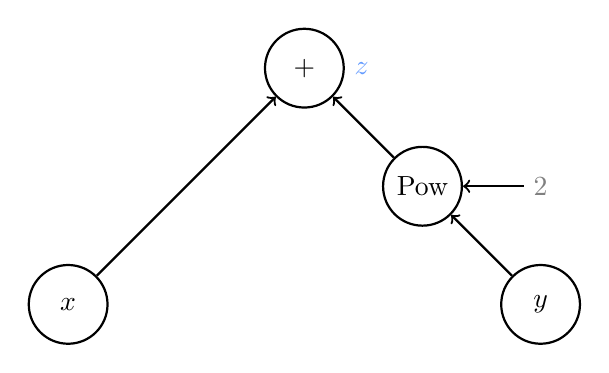
\begin{tikzpicture}
  [
    Round/.style={circle, draw=black!, fill=green!0, thick, minimum size=10mm},
    Red/.style={circle, draw=black!, fill=red!255, thick, minimum size=10mm},
    Yellow/.style={circle, draw=black!, fill=yellow!255, thick, minimum size=10mm}
  ]
  % Nodes
  \node[Round, label=right:{\textcolor{charlesBlue}{$z$}}] (v5) at(-3, -4.5) {$+$};
  \node[Round] (v4) at(-1.5, -6) {Pow};
  \node (v3) at(0, -6) {\textcolor{gray}{$2$}};
  \node[Round] (v2) at(0, -7.5) {$y$};
  \node[Round] (v1) at(-6, -7.5) {$x$};

% Lines
  \path [->, draw, thick] (v4) -- (v5);
  \path [->, draw, thick] (v1) -- (v5);
  \path [->, draw, thick] (v3) -- (v4);
  \path [->, draw, thick] (v2) -- (v4);
  
  \end{tikzpicture}
  \end{center}
  \caption{Topological graph for the programing statement \texttt{z = x + pow(y, 2)}}
  \label{fig:ad}
  \end{figure}
  
  We now take the perspective, not of a modeler, but of a developer.
  %
  Let $q \in \mathbb{R}^n$ be parameters and $x \in \mathbb{R}^k$ fixed data. 
  For AD to work, a function in \texttt{Stan}, $f: \mathbb{R}^{n + k} \mapsto \mathbb{R}^m$, 
  must compute the output, $f(q, x)$, and the $n \times m$ Jacobian matrix, $J$, 
  where $J_{ij} = \partial f_i / \partial q_j$.
  %
  This can be done in two ways: either we explicitly code a method to compute $J$,
  in which case our function behaves as a node on the expression graph;
  or we express $f$ in terms of other \texttt{Stan} functions and directly use AD. 
  The latter method is by far the easiest one to implement.
  Unfortunately, it can lead to inefficient and unstable code, when recklessly applied
  to complex mathematical functions. Two relevant examples are numerical solvers for
  ODEs and algebraic equations.
%  How \texttt{Stan} deals with these cases is respectively discussed in \cite{Carpenter:2015}
%  and \cite{Margossian:2018}.
  
  At a \texttt{C++} level, AD (as implemented in \texttt{Stan}) requires a new class, \texttt{var}, which
  contains (1) the value of a variable and (2) its adjoint with respect to the log 
  joint distribution. Recall the adjoint of $x$ with respect to $f$ is the derivative of $f$
  with respect to $x$. There is therefore an important distinction between parameters,
  with respect to which we need to calculate the gradient and 
  which must therefore be coded as \texttt{var}, and data, which are more simply 
  coded as \texttt{double}.

 It is good practice to allow users to call a function with only fixed data arguments.
 Most of the time, this means that arguments which may be parameters are templated, 
 and can be passed as either \texttt{double} or \texttt{var} objects.
 For more details on how to write new functions in \texttt{Stan} at a \texttt{C++}
 level, see the entry \textit{Contributing new Stan functions}, 
 on \url{https://github.com/stan-dev/stan/wiki/}.
 
 \section{Ordinary differential equations in pharmacometrics}
  
  The section is, in part, adapted from a presentation we gave at the 2017 Stan 
  Conference on \textit{Differential Equation Based Models in Stan} \cite{Margossian:2017}.
  
  ODEs are a powerful tool to describe physical and biological processes.
  They persevere across disciplines and keep arising in a remarkable fashion.
  They are central to pharmacometrics and by extension to \texttt{Torsten}. 
  While they can be given several physical interpretations, their mathematical properties 
  are common to all problems, which allows us to develop general purpose tools.

  \subsection{When do ordinary differential equations arise?}

  We deal with an ordinary differential equation (ODE) when we want to determine a
  function $y(t)$ at a specific time but only know the derivative of that function, $\mathrm{d}y/\mathrm{d}t$.
  In other words, we know the rate at which a quantity of interest changes but not the quantity 
  itself. In many scenarios, the rate depends on the quantity itself.

  To get a basic intuition, consider the example of a gas container with a hole in it  
  (figure~\ref{GasContainer}). We can think of the gas as being made of molecules that move 
  randomly in the container. Each molecule has a small chance of leaking through the hole. Thus
  the more molecules inside the container, the higher the number of escaping molecules per unit
  time. If there are a large number of molecules and the gas behaves like a continuous fluid, we
  observe that the more gas in the container, the higher the leakage. This statement can be 
  written as the differential equation:
  %
  $$ \frac{dy}{dt} = -ky(t)$$
  %
  where $y$ is the amount of gas in the container and $k$ is a positive constant. Note
  that $y' = \mathrm{d}y/\mathrm{d}t$ is an acceptable notation.

\begin{figure}[!htb]
\begin{center}
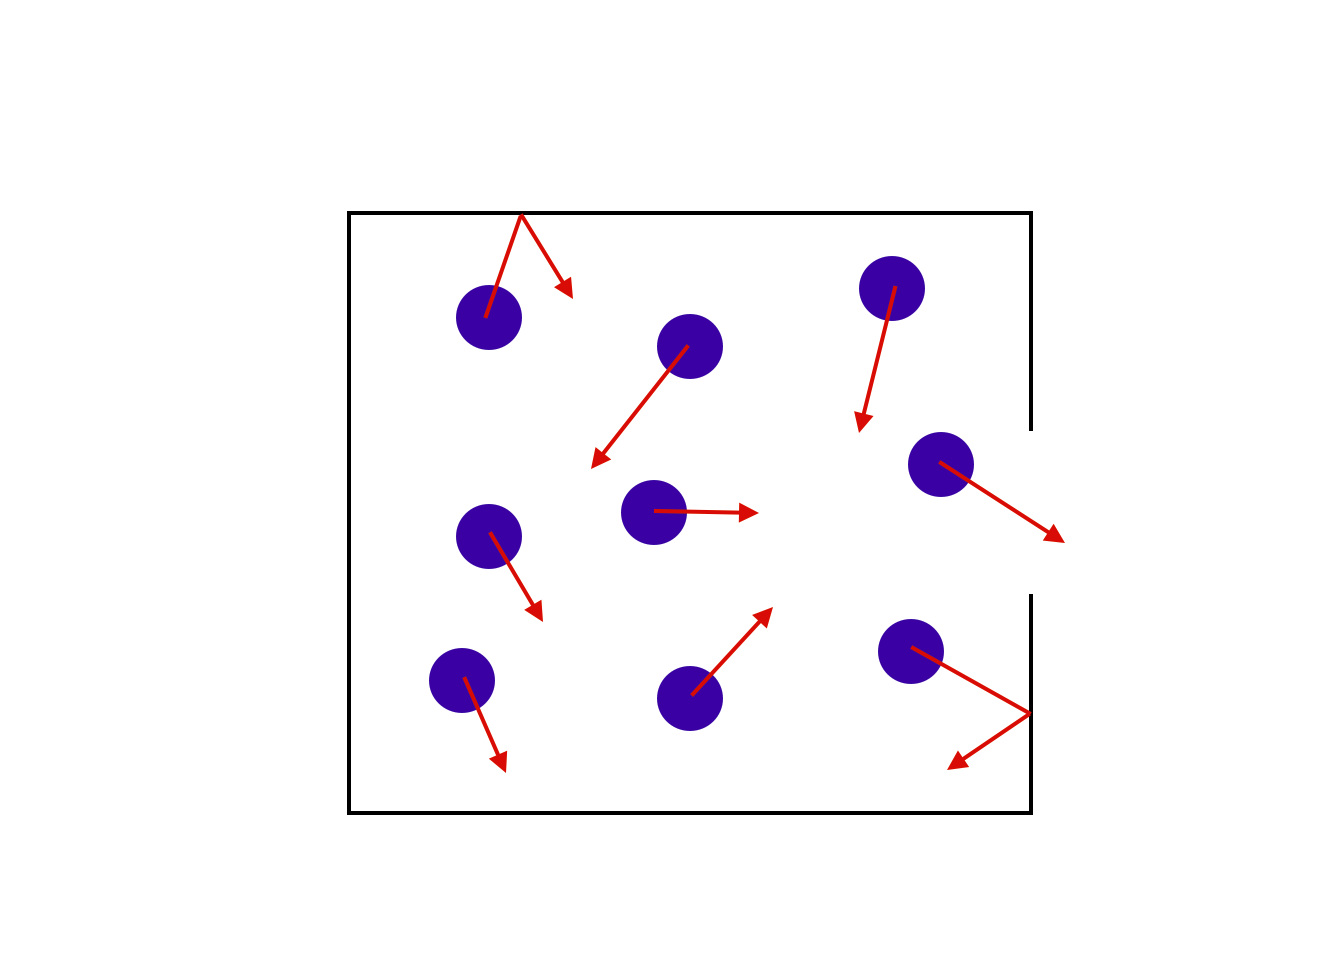
\includegraphics[width=3.0in,trim=0in 0in 0 0in]{graphics/GasInBox.png}
\caption{{Gas container with a hole. \textit{Gas molecules in a box move in a (approximatively)
random fashion. In the limit where we have a lot of particles and the gas behaves like a 
continuous fluid, the rate at which the gas leaks is proportional to the amount of gas in the container.
This physical process is described by the differential equation $ \mathrm{d}y/\mathrm{d}t = -ky(t)$, 
where $y$ is the amount of gas in the container.}}}
\label{GasContainer}
\end{center}
\end{figure}

  In a pharmacokinetic-pharmacodynamic (PK/PD) compartment model, we treat physiological
  components, such as organs, tissues, and circulating blood, as compartments between which
  the drug flows and/or in which the drug has an effect. A compartment may refer to more than  
  one physiological component. For example, the central compartment typically consists of the 
  systemic circulation (the blood) plus tissues and organs into which the drug diffuses rapidly.

  Just like our leaking gas in a container, the rate at which the quantity of drug changes depends
  on the drug amount in the various compartments (in the limit where the drug behaves like a 
  continuous substance). Things are slightly more complicated because instead of one box, 
  we now deal with a network of containers. This results in a system of ordinary differential equations.
  
  \subsection{An example: ODE system for the Two Compartment Model}
  
Consider the common scenario in which a patient orally takes a drug. The drug enters the body
through the gut and is then absorbed into the blood. From there it diffuses into and circulates back
and forth between various tissues and organs. Over time, the body clears the drug, i.e. the drug exits 
the body (for instance through urine)  (figure~\ref{TwoCptNice}).

Our model divides the patient's body into three compartments:
\begin{itemize}
  \item \textbf{The absorption compartment}: the gut
  \item \textbf{The central compartment}: the systemic circulation (blood) and tissues/organs 
  into which the drug diffuses rapidly
  \item \textbf{The peripheral compartment}: other tissues/organs into which the drug 
  distributes more slowly
\end{itemize}

We conventionally call this a \textit{Two Compartment Model}, which may seem odd since
 the model has three compartments. The idea is that the ``absorption compartment" doesn't
 really count. We adopt this convention mostly to agree with the community.
%
We describe the drug absorption using the following differential equations:
%
\begin{eqnarray}
  \begin{aligned}
  y_\mathrm{gut}' &= -k_a y_\mathrm{gut} \\
  y_\mathrm{cent}' &= k_a y_\mathrm{gut} - \left(\frac{CL}{V_\mathrm{cent}} + \frac{Q}{V_\mathrm{cent}} \right) y_\mathrm{cent} +  \frac{Q}{V_\mathrm{peri}} y_\mathrm{peri} \\
  y_\mathrm{peri}' &= \frac{Q}{V_\mathrm{cent}} y_\mathrm{cent} - \frac{Q}{V_\mathrm{peri}} y_\mathrm{peri}
  \end{aligned}
  \label{eq:2Cpt}
\end{eqnarray}
%
with \\
$y_\mathrm{gut}$ : the drug amount in the gut (mg)  \\
$y_\mathrm{cent}$ : the drug amount in the central compartment (mg)  \\
$y_\mathrm{peri}$ : the drug amount in the peripheral compartment (mg)  \\
$k_a$ : the rate constant at which the drug flows from the gut to the central compartment ($h^{-1}$)  \\
$Q$ : the clearance at which the drug flows back and forth between the central and the peripheral compartment (L/h) \\ 
$CL$ : the clearance at which the drug is cleared from the central compartment (L/h)  \\
$V_\mathrm{cent}$ : the volume of the central compartment (L)  \\
$V_\mathrm{peri}$ : the volume of the peripheral compartment (L) \\

\begin{figure}[!htb]
\begin{center}
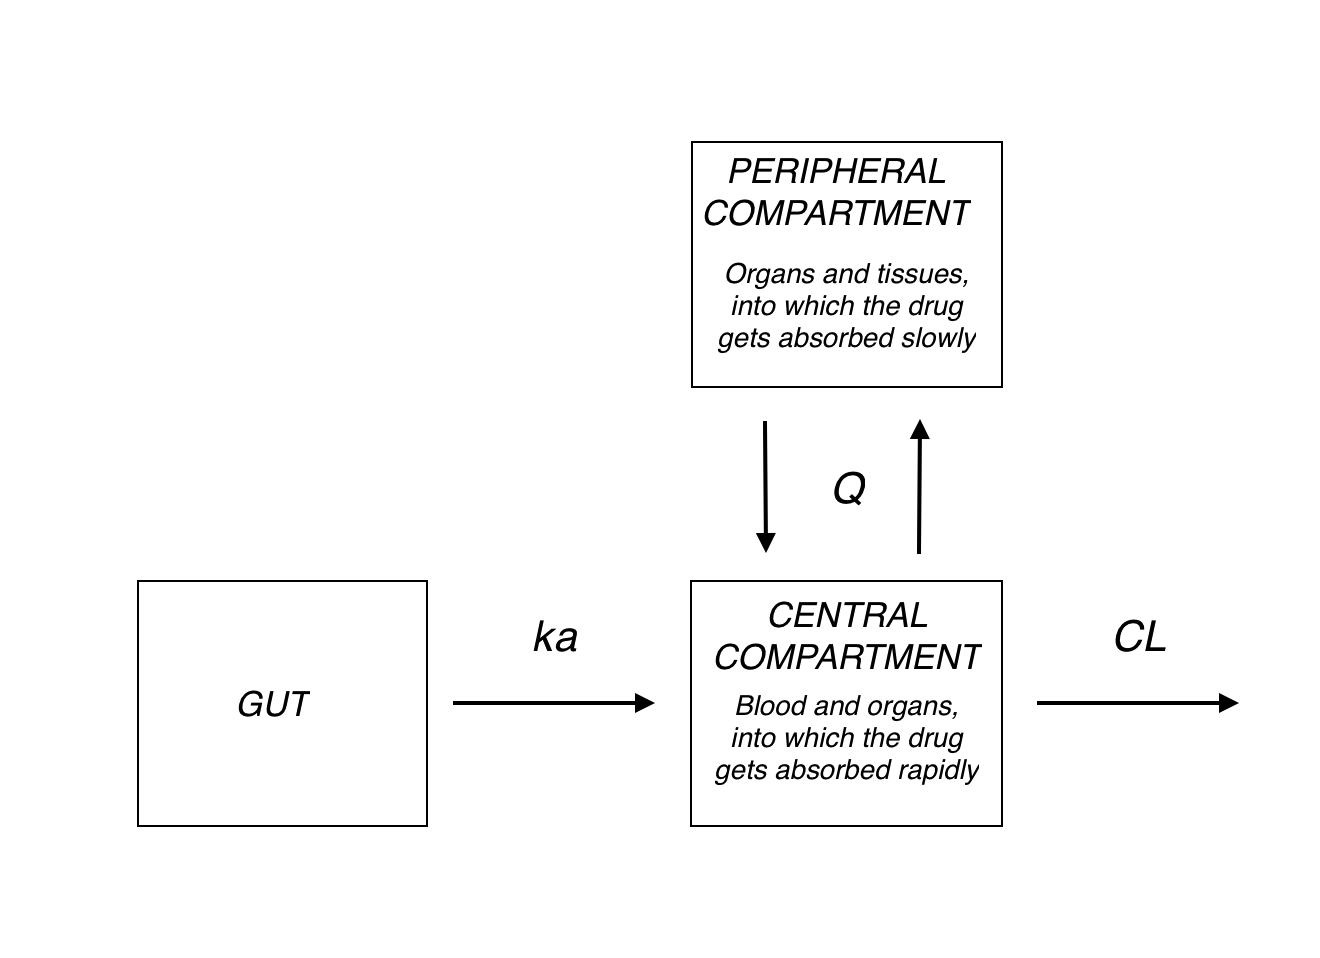
\includegraphics[width=4in,trim=0in 0in 0 0in]{graphics/TwoCptNice.png}
\caption{{Two Compartment Model. \textit{An orally administered drug enters the body through
the gut and is then absorbed into the blood, organs, and tissues of the body, before being cleared out.}}}
\label{TwoCptNice}
\end{center}
\end{figure}

\subsection{Overview of tools for solving differential equations}

Solving ODEs can be notoriously hard.
%
In the best case scenario, an ODE system has an analytical solution we can hand-code
(as we have done for the one and two compartment models). The vast majority of times,
we need to approximate the solution numerically. There exists a very nice technique, 
involving matrix exponentials, for solving linear ODEs. Nonlinear systems are significantly 
more difficult but fortunately we can tackle these problems with numerical integrators.

Specialized algorithms for solving ODEs tend be more efficient but have a narrower application; 
the reverse holds for more general tools. We provide both, thereby allowing users to tackle a 
broad range of problems and optimize their model when possible  (figure~\ref{DiffEqTools}).

\begin{figure}[!htb]
\begin{center}
\includegraphics[width=5in,trim=0in 0in 0 0in]{graphics/ODEsolvers_ext.png}
\caption{{The ``Optimized-Applicable Spectrum" of tools for solving ODEs. \textit{The top 
line gives the technique to solve differential equations, the next line the type of ODE 
system this method should be applied to, and the third line (blue) an example from 
pharmacometrics, discussed in the user manual. Modelers should prefer the left-most 
applicable technique.}}}
\label{DiffEqTools}
\end{center}
\end{figure}

\subsection{The Event schedule}

\subsubsection{Handling exterior interventions}

The ODE system only describes the natural evolution of the patient's system, that is 
how the drug behaves once it is already in the body. Describing this natural evolution, 
by solving ODEs, is the task of the \textit{evolution operator}. This operator does not 
account for exterior interventions during the treatment, such as the intake of a drug 
dose. To be accurate, our model must compute these exterior events and solve ODEs
in the context of an \textit{event schedule}.

We follow the convention set by NONMEM\textregistered\footnote{NONMEM\textregistered\ 
is licensed and distributed by ICON Development Solutions.}, which is popular amongst 
pharmacometricians and which we find acceptable.

An event can either be a change in the state of the system or the measurement of a certain 
quantity. We distinguish two types of events:
\begin{enumerate}
  \item \textbf{State Changer}: an (exterior) intervention that alters the state of the 
  system (for example, a bolus dosing, or the beginning of an infusion)
  \item \textbf{Observation}: the measurement of a quantity of interest at a certain time
\end{enumerate}

Between two subsequent events, the ODEs fully describe the PK/PD system. Knowing 
the state $y_0$ at time $t_0$ fully defines the solution at finite times. Exploiting this 
property, \texttt{Torsten} calculates amounts in each compartment from one event to the other.
 The initial conditions of the ODEs are specified by the previous event and the states 
 evolved from $t_\mathrm{previous}$ to $t_\mathrm{current}$.

The user passes the event schedule using a data table. 
%
NONMEM's convention allows one row to code for multiple events. For example, a 
single row can specify a patient receives multiple doses at a regular time interval. Consider: \\
%
\texttt{TIME = 0, EVID = 1, CMT = 1, AMT = 1500, RATE = 0, ADDL = 4, II = 10, SS = 0} \\
%
This row specifies that at time 0 (\hbox{TIME = 0}), a patient receives a 1500 mg 
(\hbox{AMT = 1500}) drug dose (\hbox{EVID = 1}) in the gut (\hbox{CMT = 1}), and will 
receive an additional dose every 10 hours (\hbox{II = 10}) until the patient has taken a 
total of 5 doses (\hbox{ADDL = 4}, being the number of additional doses, + 1, the original 
dose). Such an event really corresponds to 5 dosing events. \texttt{Torsten} augments the event 
schedule accordingly, before solving the ODEs recursively from one event to the other.
%
In summary, each \texttt{Torsten} function:
\begin{enumerate}
  \item augments the event schedule to include all state changers
  \item calculates the amounts in each compartment at each event of the augmented schedule by
  \begin{enumerate}
    \item integrating the ODEs and computing the \textit{natural} evolution of the system
    \item computing the effects of state changers
  \end{enumerate}
  \item returns the amounts at each event of the original schedule.
\end{enumerate}

\subsubsection{Dosing events}

Most state changers in pharmacometrics (though by no means all of them) are due to drug
intakes. A drug can be administered using a bolus intake or an infusion over a finite time.

To compute a bolus dose, \texttt{Torsten} simply adds the administered dose amount to the drug 
mass, $y(t)$, and then resumes integrating the ODEs. Letting $f(y, t) = y'(t)$ be the right-hand 
side of our ODE system, $m$ the administered amount and $\tau$ the time of the dosing, we get:
%
\begin{eqnarray}
  \begin{aligned}
  y(\tau ^ +) &= y(\tau^-) + m \\
  y(t) &= \int_{\tau ^ +} ^ t f(y, t') dt'
  \end{aligned}
\end{eqnarray}
%
The bolus dosing event introduces a discontinuity with respect to time (figure~\ref{fig:bolus}).
As we will discuss in a moment, this can lead to issues.

Alternatively, a drug may be administered via infusion.
Users code for an infusion by setting a non-zero rate. For example,  \\
\hbox{\texttt{\{AMT = 1200, RATE = 150, ...\}}} corresponds to an infusion of 150 unit mass per unit
time that will last 8 unit time (leading to a total of 1200 unit mass being administered). \texttt{Torsten} handles
this scenario by creating a new event at the end of the infusion time. For all events between the
beginning and end of the infusion, the rate in each compartment is augmented by the infusion rate,
$R$. Letting $\tau$ be the beginning, and $\delta$ the end of the infusion time, we get:
%
\begin{eqnarray}
  \begin{aligned}
  y(\delta) &= \int_\tau ^ \delta f(y, t') + R dt' \\
  y(t) &= \int_\delta ^ t f(y, t') dt'
  \end{aligned}
\end{eqnarray}
%
Note the upper-bound of the integral, $\delta = m / R$, can be a latent parameter if either $m$ or
$R$ is a parameter. In other words, we may need to compute $\partial y / \partial \delta$. This will
be relevant to our discussion on numerical integrators.

\begin{figure}[!htb]
\begin{center}
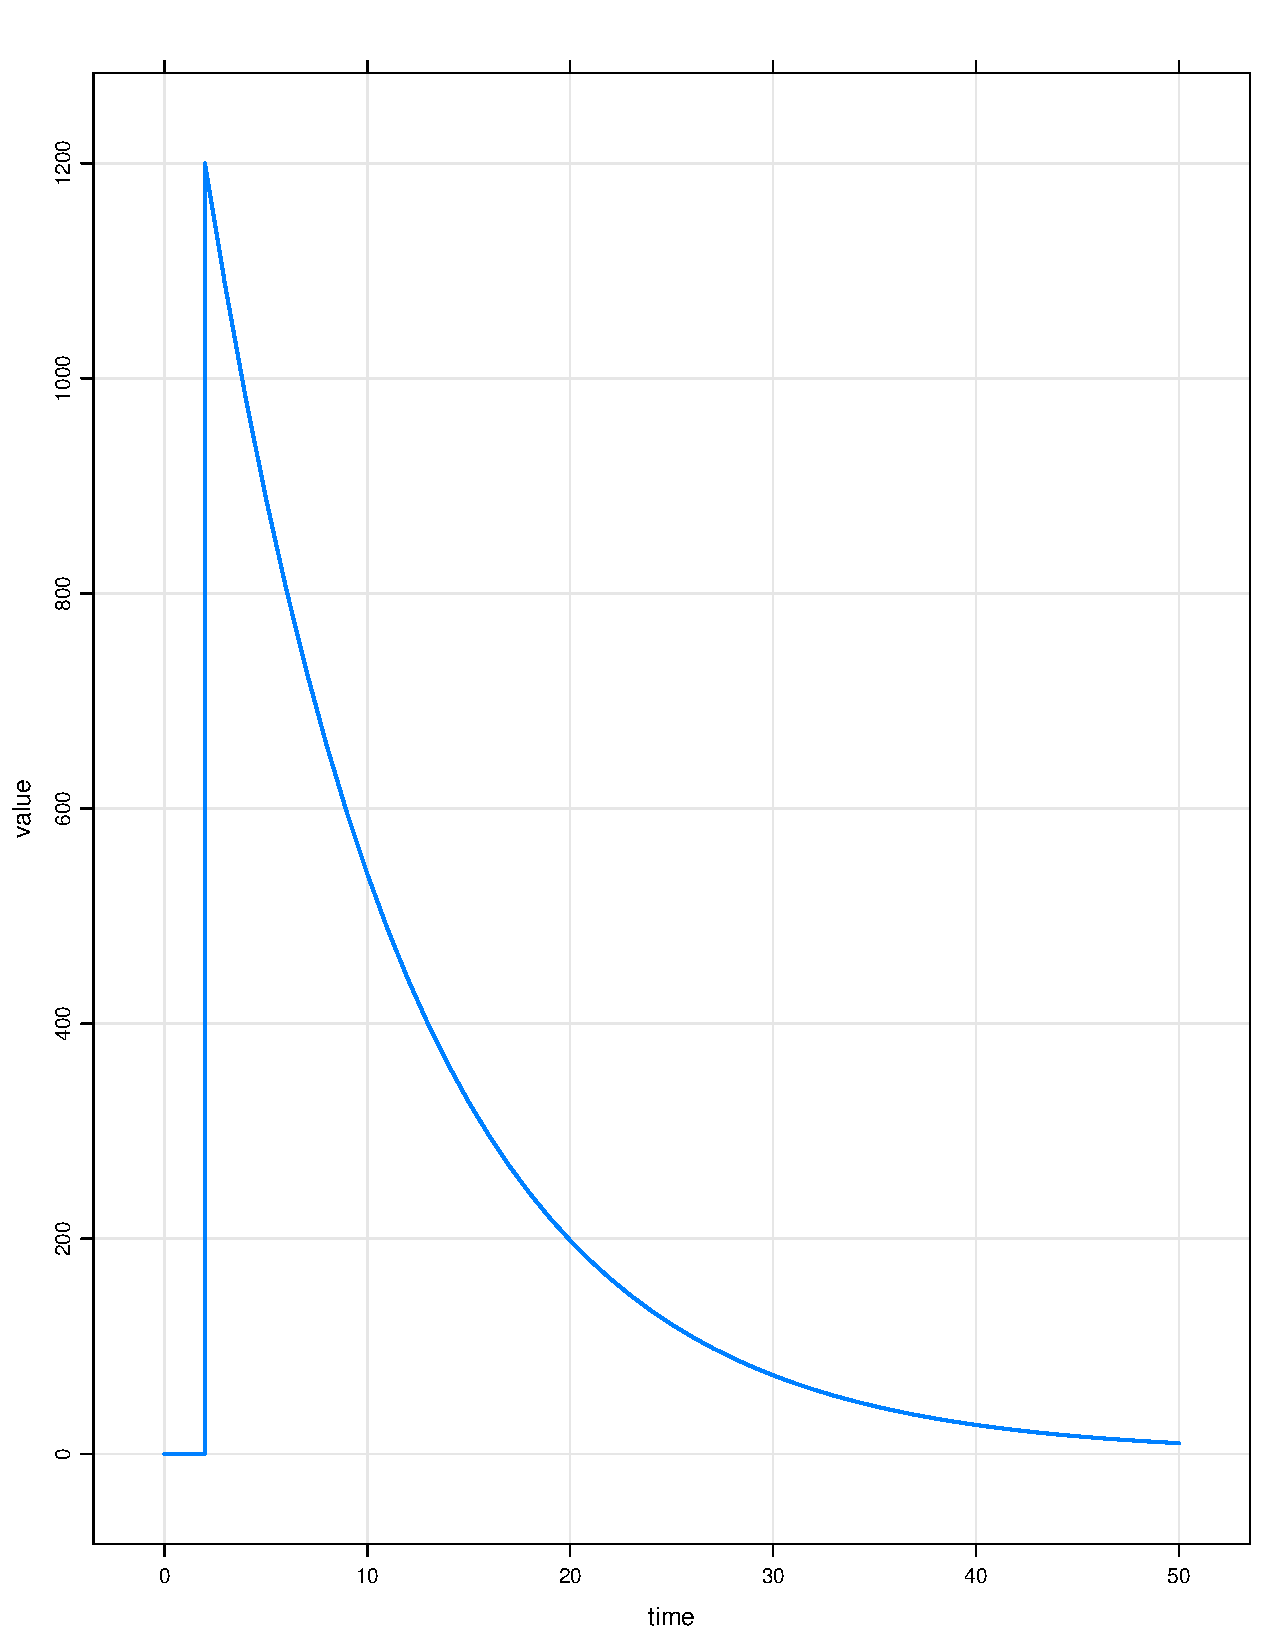
\includegraphics[width = 2.5in, height = 2.5in, trim=0in 0in 0 0in]{graphics/BolusDose.pdf}
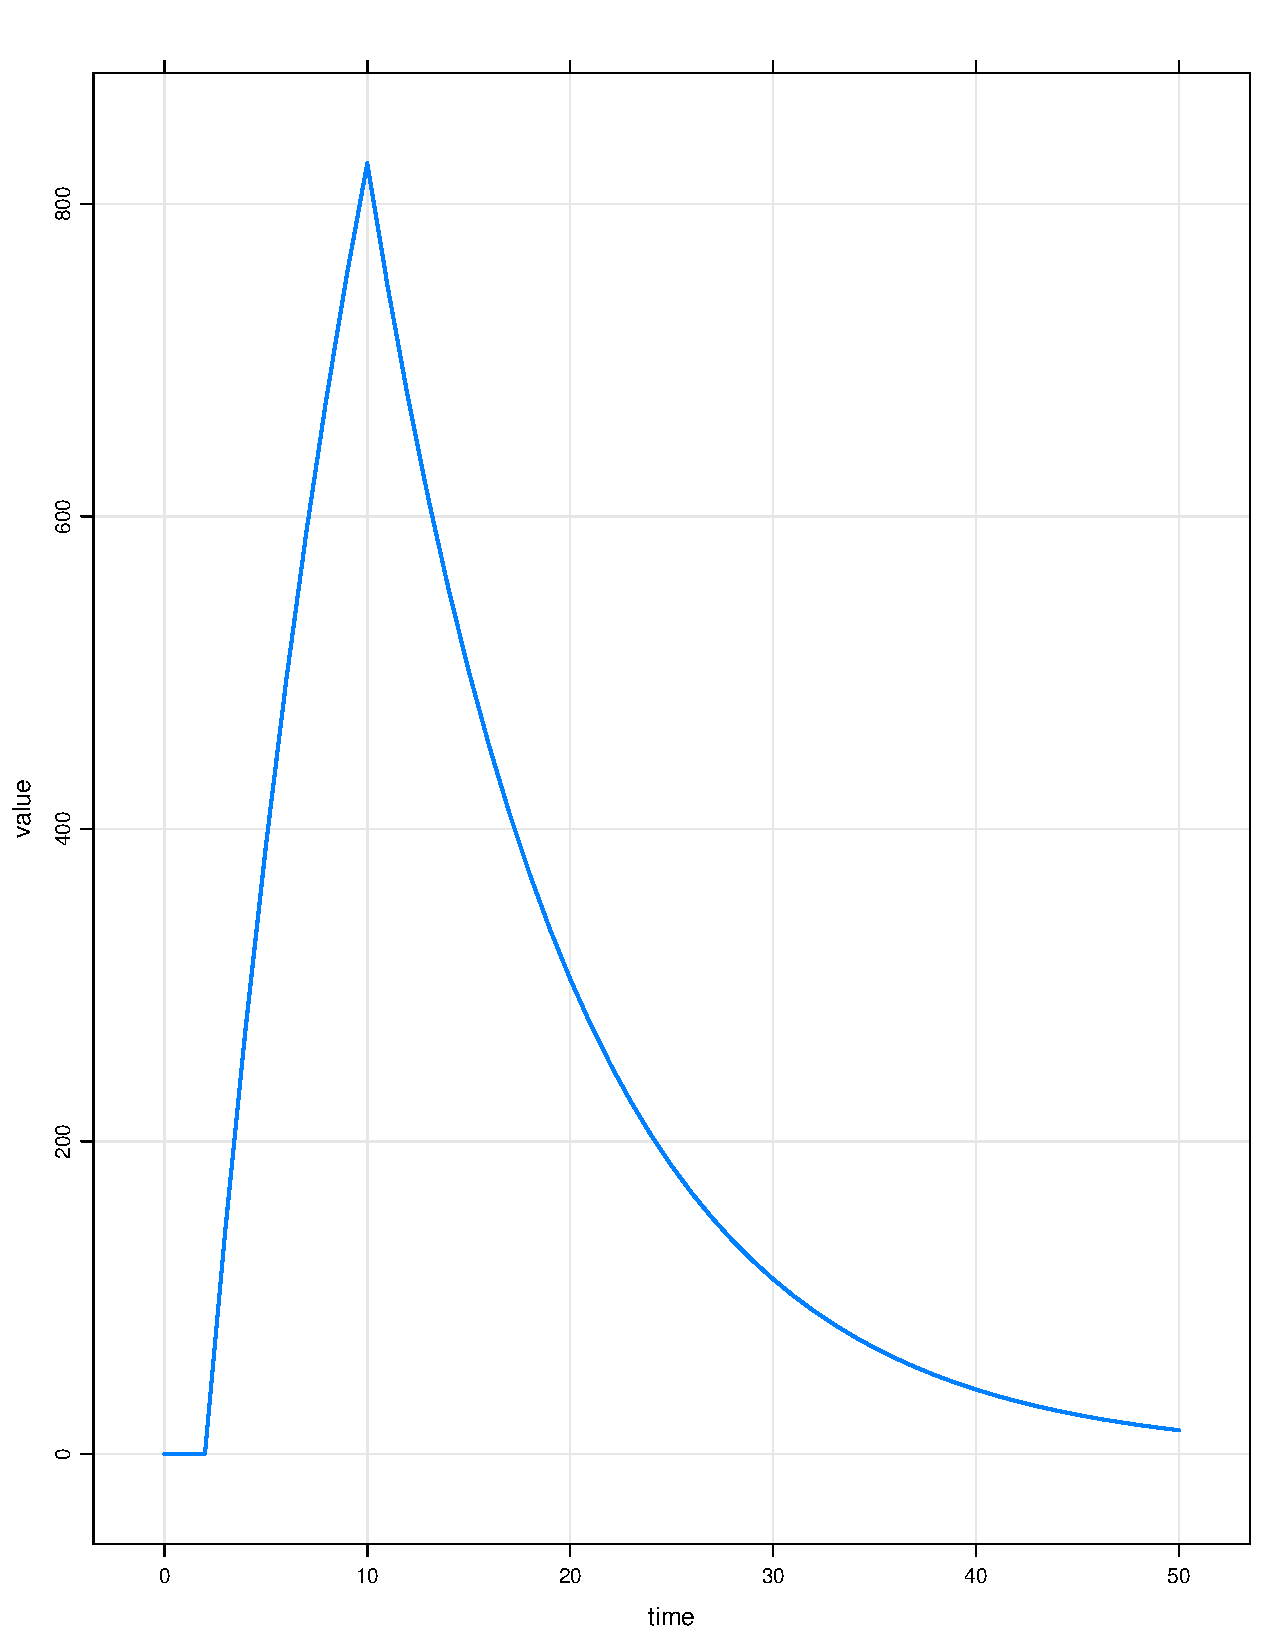
\includegraphics[width = 2.5in, height = 2.5in, trim=0in 0in 0 0in]{graphics/Infusion.pdf}
\caption{Simulated drug mass in a patient's gut after an oral drug administration 
\textit{\hbox{\textbf{(left)} At} $t = 2 \mathrm{h}$ a patient receives a $1200 \mathrm{mg}$
bolus dose. This creates a discontinuity in the drug mass, $y(t)$. This can be an issue
when $t_\mathrm{lag}$ is a parameter. As the system evolves, 
the drug gets naturally cleared out of the gut and absorbed into the blood and other organs (see 
equation~\ref{eq:2Cpt}).  \textbf{(right)} A patient receives an infusion, starting at $t = 2\mathrm{h}$
at a rate of $R = 150\mathrm{mg/h}$. After 8 hours, the infusion stops and the drug mass decreases.
Figures generated with \texttt{mrgsolve}.}} 
\label{fig:bolus}
\end{center}
\end{figure}

Let us now go back to bolus doses, and issues they may cause.
If $\tau$ or any observation time depends on one or 
more model parameters,
the joint distribution of our model may no longer be differentiable at every point
of interest.
This problem arises, for example, when the modeler tries to estimate \textit{lag times}.
%
We still need to characterize how important the resulting error is\footnote{see issue \#3 on 
\url{github.com/metrumresearchgroup/math/issues/3}.}. We tested the computation of the Jacobian matrix
with AD. 
As expected, the derivative is not properly evaluated  at events which occur \underline{exactly} at the time 
of a dosing, lag time accounted for.
To be more precise, the derivatives are ill-defined, and can at best be characterized by
looking at two one sided limits.
The main concern here is then not the value that AD returns, but the fact that it
does not identify the derivative as being ill-posed and return an error message to that effect.
In that sense, AD is not robust.

But back to our problem in pharmacometrics: lag times are continuous variables, therefore 
a scenario in which an event occurs exactly at the time of the dosing  is unlikely
(in many settings, such a scenario has in fact a probability 0). 
%
Our test further reveals the Jacobian matrix at other events is properly 
evaluated\footnote{There may still be issues with numerical solvers. This has not yet been tested for.}.
An additional mitigating factor is that we usually do not make measurements on the absorption
compartment but on central compartments. 
In such compartments, the change in drug mass is not instantaneous.
They introduce a discontinuity in derivatives, but this is not an issue.



\subsubsection{Model parameters}\label{modelParms}

In addition to passing the event schedule to a \texttt{Torsten} function, modelers must specify the 
\textit{model parameters}:
\begin{itemize}
  \item $\theta$: parameters which appear in the ODE system
  \item $F$: the bioavailability fraction, specified for each compartment
  \item $t_\mathrm{lag}$: lag times, specified for each compartment
\end{itemize}
%
All continuous variables, including elements of the event schedule, can be passed as either 
parameters or fixed data. This demand some caution when we compute sensitivities. Handling 
$\theta$ is straightforward.  $F$ and $t_\mathrm{lag}$ on the other hand modify variables which
get passed to the evolution operator and create latent parameters. In particular, $F$ modifies 
the rate, $R$, for regular solutions and the amount, $m$, for steady state solutions.
$t_\mathrm{lag}$ alters the dosing time, $t$. \ \\

\begin{center}
  \begin{tabular}{l l}
  \rowcolor[gray]{0.95} \textbf{Model Parameter} & \textbf{Latent Parameter(s)} \\
    $F$ & $R$ (non-steady state case) \\
         &  $m$  (steady state case) \\ 
  \rowcolor[gray]{0.95} $t_\mathrm{lag}$ & $t$ \\
  \end{tabular} \\
\end{center}


\section{Solving ordinary differential equations}

Recall we want to compute the log joint distribution and its gradient (equivalently,
the gradient of the log posterior). We therefore need to solve differential equations and propagate 
derivatives through them.
%
This means computing the Jacobian matrix of the solutions with
respect to the parameters. In \texttt{Torsten}, this tasks is carried out by the \textit{pred} functors,
which act as the \textit{evolution operators} (they compute the evolution of the system from
one state to the other between two events).

\subsection{Analytical solution}

We hand-code the solution for the One and Two Compartment models with a first-order
absorption. The Jacobians are computed using AD.
We could work out these derivatives analytically, but the resulting speed-up may
only be minor. 

\subsection{The Matrix Exponential}

Consider a system of \underline{linear} differential equations:
%
$$ y^\prime(t) = Ky(t) $$
%
where $K$ is a constant matrix and $y$ a vector function. The solution to the equation is given by 
%
\begin{eqnarray}
  y(t) = e^{tK} y_0
  \label{eq:linearSol}
\end{eqnarray}
%
where $y_0$ is the initial condition and $e$ is the \textit{matrix exponential}, formally defined
by the convergent power series:
%
\begin{eqnarray}
  e^{tK} = \sum_{n=0}^{\infty} \dfrac{(tK)^n}{n!} = I + tK + \frac{(tK)^2}{2} + \frac{(tK)^3}{3!} + ...
  \label{eq:matrix_exp}
\end{eqnarray}
%
Looking at this definition, we clearly see the derivative of $e^{tK}$ is $Ke^{tK}$.
In practice, it is not feasible to compute an infinite number of terms.

There exist several methods to compute the matrix exponential.
\cite{MolerAndVanLoan:2003} provide an excellent and detailed review.
\cite{Al-Mohy:2011} propose an algorithm to efficiently compute the action of the matrix exponential,
that is the product of $e^A$ with a vector, such as $y_0$\footnote{For some details on how this is
done in \texttt{Stan}, see \url{https://github.com/stan-dev/math/issues/771}.}.
Note that when solving a system of linear ODEs, the solution is the action of a matrix exponential.
To accommodate the scope of applications of the matrix exponential, \texttt{Stan} provides three routines,
summarized in table~\ref{tab:matrixExp}.
%
We review the algorithm implemented in \texttt{Stan} in some level of details
to outline certain questions that we, as developers, may ask ourselves.

\setlength{\extrarowheight}{10pt}
\begin{table}
  \begin{center}
  \begin{tabular}{l l l}
  \rowcolor[gray]{0.95} \textbf{Routine} & \textbf{Arguments} & \textbf{Output} \\
  \texttt{matrix\_exp()} & $A$ & $e^A$ \\
  \rowcolor[gray]{0.95} \texttt{matrix\_exp\_multiply()} & $A$, $B$ & $e^A B$ \\
  \texttt{scale\_matrix\_exp\_multiply()} & $A$, $B$, $t$ & $e^{At} B$ \\
  \end{tabular}
  \caption{Routines in \texttt{Stan} to compute the matrix exponential.}
  \label{MatrixExp}
  \end{center}
  \label{tab:matrixExp}
\end{table}
\setlength{\extrarowheight}{0pt}


First we note that for a $2 \times 2$ matrix
\begin{eqnarray*}
   K = \left[\begin{array}{cc}
	a & b \\
	c & d
	\end{array}\right] \\
\end{eqnarray*}
%
there is an analytical solution, provided $(a - d)^2 + 4bc > 0$ \cite{ToddWeisstein}. Naturally, we will want to take
advantage of this.
%
For the general case, we use the Pad\'e approximation coupled with scaling and squaring.
The  idea is to approximate the matrix exponential with the finite series:
%
\begin{eqnarray*}
  R_{pq}(K) &=& [D_{pq}(K)]^{-1}  N_{pq}(K)
\end{eqnarray*}
%
where
%
\begin{eqnarray}
  \begin{aligned}
  N_{pq}(K) &=& \sum_{j=0}^p \frac{(p + q - j)! p!}{(p + q)! j! (p - j)!}A^j \\
  D_{pq}(K) &=& \sum_{j=0}^q \frac{(p + q - j)! q!}{(p + q)! j! (q - j)!}(-A)^j
  \end{aligned}
  \label{eq:pade}
\end{eqnarray}
%
In the asymptotic limit, $(p, q) \rightarrow (\infty, \infty)$, we recover the  definition of the 
matrix exponential. \cite{MolerAndVanLoan:2003} explain the benefits of this method.
%
We do run into issues for large $||K||$ because of round-off errors. This is where the scaling 
and squaring comes into play. Noting the following property of the matrix exponential:
%
$$ e^K = (e^{K/m})^m $$
%
we rescale the argument of the Pad\'e approximation and exponentiate the final product 
by $m$.

All in all, this a rather nasty looking equation, with several tuning parameters, such as the choice
of $p$, $q$, and $m$. Theoretical considerations can help us make an informed decision.
Fortunately, there exist several packages which already implement this algorithm.
The \texttt{C++} library \texttt{Eigen} \cite{Eigen:2013} contains an unsupported routine to compute
the matrix exponential, using the above described method.
It is readily available to \texttt{Stan}, which extensively uses other components of \texttt{Eigen}.
It would be to look at other routines, such as the one implemented in the package \texttt{Expokit} \cite{Sidje:1998}.
Tests revealed \texttt{Eigen} usually computes 13 terms in the Pad\'e series,
whereas \texttt{Expokit} typically computes 6, yielding less precise results but faster computation.
For our goals, 6 terms may already provide us with all the accuracy we need.
More generally, the ideal number of terms depends on the matrix.

Once we have selected a method to calculating the matrix exponential,
we need to propagate derivatives by computing the derivatives of the output with respect to
the parameter-dependent inputs. This amounts to constructing a Jacobian matrix or tensor.
There are clever ways of doing this, but for \texttt{matrix\_exp()} we can actually get away
with brute force AD.
Indeed, while equation~\ref{eq:pade} looks rather intricate, it only involves basic operations
which can be sorted into an expression graph.
For a basic implementation, it therefore suffices to overload \texttt{Eigen}'s routine, such that
it can handle \texttt{var} types.
A word a caution though: in other cases, brute-forcing AD through a numerical method can
fail spectacularly, yielding unstable and inefficient code.
Two examples are numerical ODE integrators and numerical algebraic solvers.
Furthermore, analytical or semi-analytical gradients tend to produce more efficient code.

%
%The \texttt{C++} library \texttt{Eigen} \cite{Eigen:2013} contains an unsupported routine to compute the matrix 
%exponential that uses the above-described method. The order of the approximation, i.e. 
%the number of terms in the series, depends on the input matrix. We find \texttt{Eigen}'s code promptly
%goes to the $13^{\text{th}}$ order, except in very simple cases. We edit \texttt{Eigen}'s code, so that
%it may handle \texttt{var} types. The Jacobian of \texttt{matrix\_exp} is approximated by applying 
%AD to the Pad\'e approximation.
%
%\textcolor{red}{Rewrite this section to cover Yi's improvement.} 
%We can improve the current implementation of \texttt{matrix\_exp} in several ways. First, we should
%hand-code the Jacobian, potentially using recommendations by Giles \cite{Giles:2008}. We suspect 
%computing 13 terms in the Pad\'e approximation is overkill; Sidje recommends 6, which is the default 
%he implements in his package \texttt{Expokit} \cite{Sidje:1998}. We also want to take advantage of methods which 
%allow us to directly compute the action of a matrix exponential on a vector. Recall our goal is to 
%compute the solution $e^{Kt}y_0$.

\subsection{Numerical integrators}

Numerical integrators fundamentally differ from analytical and matrix exponential methods.
Rather than evaluating the solution at certain points of interest,
integrators construct the \textit{solution function}, step by step, across a large grid of points.
This is the main reason why there are much slower than the methods we have examined so far;
they however require much less assumptions about the structure of the solution and apply to a much
broader class of problems. Most importantly, they allow us to solve systems of nonlinear ODEs with
no closed-form solutions.

Euler's method provides the right intuition on how integrators work.
We begin at a point $$y_0 = y(t_0)$$
and then compute $$y_1 = y(t_0 + \Delta t)$$ by evaluating the derivative of $y$ with respect to $t$
at $y_0$ and performing a \textit{tangent approximation}.
Recall the ODEs give us the needed derivatives.
We then repeat this procedure, starting at point $y_1$, and computing a tangent there.
The output is a piece-wise linear approximation of the true solution.
The immediate question is: what step size, $\Delta t$, should we use?
Again, we want to achieve accuracy, but also minimize computational cost.

This problem is notoriously hard when we deal with \textit{stiff} systems.
Stiffness is not a rigorously mathematically defined property but nevertheless captures an important
idea. In a stiff equation, the rate at which $y$ changes with respect to $t$
varies dramatically from one region
to the other. Hence a given step size may be optimal in one region, but very suboptimal
in another region. Tackling this issue requires its own class of algorithms which can adaptively
change the step size, as the solution gets computed


\texttt{Stan} provides three ODE integrators. The Runge-Kutta $4^\mathrm{th}/5^\mathrm{th}$ order, \\
\texttt{integrate\_ode\_rk45}, is relatively fast but cannot handle stiff ODEs.
For stiff systems, modelers should use \texttt{integrate\_ode\_bdf} or \texttt{integrate\_ode\_adams},
which respectively implement the backward differentiation method and the Adams-Moulton schemes.
The latter is more stable when we wish to achieve higher-order accuracy.
Note that, once again, these methods fall on an optimum - applicable spectrum.


\subsubsection{Propagating derivatives through an ODE system}

Suppose our solution is $y \in \mathbb R^n$. 
We first need to identify inputs which may depend on model parameters.
These can be:
%
\begin{enumerate}
  \item certain coefficients in the ODEs, $\theta$
  \item initial states, $y^0$
  \item time points, $t$
\end{enumerate}
%
Correspondingly, we need to construct the Jacobian matrix
%
\begin{eqnarray*}
     J = \left[\begin{array}{c c c c c c c c c c}
	  \frac{\partial y_1}{\partial \theta_1} & . . . & \frac{\partial y_1}{\partial \theta_p} & \frac{\partial y_1}{\partial y_1^0} &...& \frac{\partial y_1}{\partial y_n^0} & ... &  \frac{\partial y_1}{\partial t_1} & ... & \frac{\partial y_1}{\partial t_k} \\
	    . . . & . . . & . . . & ... & ... & ... & ... & ... & ... & ... \\
	  \frac{\partial y_n}{\partial \theta_1} & . . . & \frac{\partial y_n}{\partial \theta_p} & \frac{\partial y_n}{\partial y_1^0} &...& \frac{\partial y_n}{\partial y_n^0} & ... &  \frac{\partial y_n}{\partial t_1} & ... & \frac{\partial y_n}{\partial t_k}
	\end{array}\right] 
\end{eqnarray*}
%
Note this matrix can be split into three components: the derivatives with respect to $\theta$, those with respect to $y^0$,
and those with respect to $t$. In practice, we may only require one of these components.
With careful coding, we only compute the derivatives we care about and keep our code efficient.

Here, a naive implementation of AD fails spectacularly.
The main reason is that, in order to compute a solution, a numerical integrator takes thousands,
if not millions of steps.
The resulting expression graph is therefore extremely large, resulting in slow, memory intensive,
and numerically unstable code.

Fortunately, there is structure in our problem which we can take advantage of.
Denote $\alpha = (\theta, y^0, t)$ the vector which contains all the elements that require sensitivities.
To obtain the needed derivatives, we augment the original ODE system with the state variables:
\begin{eqnarray*}
J_{ij} = \frac{\partial}{\partial \alpha_j}y_i
\end{eqnarray*}
%
which correspond to the individual elements of the Jacobian matrix.
The resulting \textit{coupled} ODE system is
%
  \begin{eqnarray*}
    y_1' & = & f_1(y, t, \theta) \\
    y_2' & = & f_2(y, t, \theta) \\
    & ... & \\
    \frac{\mathrm d}{\mathrm d t} \frac{\partial y_1}{\partial \theta_1} & = & f_{1,1}(y, t, \theta) \\
    & ... &  \\
    \frac{\mathrm d}{\mathrm d t} \frac{\partial y_n}{\partial \theta_p} & = & f_{n, p}(y, t, \theta) \\
    & ... &  \\
    \frac{\mathrm d}{\mathrm d t} \frac{\partial y_1}{\partial y_1^0} & = & f_{n, p}(y, t, \theta)  \\
    & ... & \\
\end{eqnarray*}
%
By solving this system, we simultaneously produce the desired solution \textit{and} the needed derivatives!
Note further that writing this system does not require an analytical form for $J_{nm}$,
but for
%
\begin{eqnarray*}
  \frac{\mathrm d}{\mathrm dt} J_{ij} & = & \frac{\mathrm d}{\mathrm dt}  \frac{\partial}{\partial \alpha_j}y_i \\
     & = &  \frac{\partial}{\partial \alpha_j} \frac{\mathrm d}{\mathrm dt} y_i
\end{eqnarray*}
%
Intuitively, we may assume that since $\frac{\mathrm d}{\mathrm dt} y_i$ is known, we can analytically
work out the derivative of the solution with respect to $\alpha_i$.
This requires some algebra; details can be found in section 13 of \cite{Carpenter:2015}.

An analysis of the augmented system shows the computational cost scales up significantly 
with the number of original states in the system; and (to a lesser degree) with the number 
of parameters. In most cases, the modeler has no control over the dimension 
of $y$. We will treat an important exception in the next section. Keeping the number of parameters
 at a minimum is a matter of careful coding.

In Stan, the functor which defines an ODE system, must observe a strict signature: \\ \\
% 
\texttt{real[] foo (real t,  {\ \ \ \ \ \ \color{gray}// time} \\
\phantom{real[] foo (}real[] y, {\ \ \ \ \color{gray}// array of states} \\
\phantom{real[] foo (}real[] theta, {\color{gray}// array of parameters} \\
\phantom{real[] foo (}real[] x\_r, {\ \  \color{gray} // array of real data} \\
\phantom{real[] foo (}int[] x\_i) {\ \ \ \color{gray} // array of integer data}
                   } \\ \\
%
This strict signature requires some careful bookkeeping, as we need to sort out which 
variables are parameters or fixed data. As we saw in section~\ref{modelParms}, it
may not be immediately obvious if a variable is a latent parameter.

\subsection{Mixed solvers: combining analytical and numerical solutions}

In certain cases, an ODE system can be split into two:
%
\begin{eqnarray*}
  \begin{aligned}
  y_1(t)' &= f_1(y_1, t) \\
  y_2(t)' &= f_2(y_1, y_2, t) \\
  \end{aligned}
\end{eqnarray*}
%
where $y_1$ does \underline{not} depend on $y_2$. In this situation, we usually refer to $y_1$
as the \textit{forcing function}. If $y_1$ has a closed-form solution, we can use a \textit{mixed solver} 
to solve the system. The idea is to solve for $y_1$ analytically and then 
numerically integrate a \textit{reduced system} to find $y_2$. This requires we write $f_2$ in 
terms of the solution $y_1$ -- often a relatively complex expression -- rather than as an 
expression of the (more simple) derivative $y_1'$. 

The mixed solver thus presents a trade-off: it increases the complexity of the integrant 
but reduces the number of states we integrate numerically. We conjecture the benefit usually outweights 
the cost, particularly with AD. The gain in efficiency varies on a case-by-case 
basis. For the example of a Friberg-Karlsson model, the average speed-up is $49 \pm 14 \%$
 \cite{Margossian:2017b}.

A proper implementation of the mixed solver requires a hand-coded closed-form solution for $y_1$ 
and some careful bookkeeping. In \texttt{Torsten}, we take advantage of the built-in solution for the one and 
two compartment models. The user is required
to specify which PK forcing function he or she wishes to use and codes the reduced system. 
\texttt{Torsten} then follows the following coding scheme: \\ \\
%
\texttt{y\_1 = f\_1; \\
y\_2 = integrate(f\_2); \\
return y = \{y\_1, y\_2\}; \\
  } \\ \\
%
where \texttt{f\_1} is the analytical solution and \texttt{f\_2} a \texttt{C++} functor which wraps the reduced
system the user passes to the \texttt{Torsten} function and observes the strict signature required by Stan's
built-in integrators. For the case of a One Compartment model forcing function, the wrapper follows 
the following coding scheme: \\ \\
%
\texttt{real[] foo(real t, \\
\phantom{real[] foo(}real[] y \\
\phantom{real[] foo(}real[] theta,  \\
\phantom{real[] foo(}real[] x\_r, \\
\phantom{real[] foo(}int[] x\_i) \{ \\
%
 \phantom{  } \textcolor{gray}{// Get PK parameters} \\
 \phantom{  } thetaPK[0] = theta[0];  \textcolor{gray}{// CL} \\
 \phantom{  } thetaPK[1] = theta[1];  \textcolor{gray}{// VC} \\
 \phantom{  } thetaPK[2] = theta[2];  \textcolor{gray}{// ka} \\ \ \\
% 
 \phantom{  } \textcolor{gray}{// Get initial PK states} \\
 \phantom{  } \textcolor{gray}{// The last two components of theta should contain the initial PK states} \\
 \phantom{  }  init\_pk[0] = theta[theta.size() - 2]; \\
 \phantom{  }  init\_pk[1] = theta[theta.size() - 1]; \\ \ \\
%  
 \phantom{  }  \textcolor{gray}{// The last element of x\_r contains the initial time} \\
 \phantom{  }  dt = t - x\_r[x\_r.size() - 1]; \\ \ \\
% 
 \phantom{  }  y\_pk = fOneCpt(dt, thetaPK, init\_PK, x\_r); \\
 \phantom{  }  dydt = \textcolor{red}{f0}(dt, y, y\_pk, theta, x\_r, x\_i); \\ \ \\
%  
 \phantom{  }  return dydt; \\
\}
} \\ \\
%
where \texttt{\textcolor{red}{f0}} is the reduced system the user provides. The reduced 
system accepts an additional argument, which allows us to pass the analytical solution \texttt{y\_pk}. 
\texttt{Torsten} takes care of the following bookkeeping tasks under the hood:
\begin{itemize}
  \item augmenting the array of parameters, \texttt{theta}, with the initial conditions for the forcing function.
  \item augmenting the array of data, \texttt{x\_r} with the initial time, so that the evolution operator
  for the forcing function, \texttt{fOneCpt}, knows between which times to evolve the forcing system.
\end{itemize}
%
These considerations extend to the case of a Two Compartment forcing function. We need to apply 
similar thinking when we deal with non-zero rates and steady state solutions.

\subsection{Rates}

The administration of a dose through an infusion alters the \textit{natural} ODE system, by 
adding a constant rate, $R$, to the derivative of the solution:
%
$$
y'(t) = f(y, t) + R
$$
%
The solution to this new ODE is worked out analytically for the One and Two compartment 
model, and for the general linear compartment model. In particular for the latter:
%
$$
y'(t) = K y(t) + R
$$
%
which gives us the solution:
%
$$
y(t) = e^{tK} (K^{-1}R + y_0) - K^{-1} R
$$ 
%
For the numerical case, the function which gets passed to the integrator is modified, by adding
 $R$ to the returned vector. If $R$ is an array of fixed data, \texttt{rate} gets passed using the argument
 \texttt{x\_r}.

If $R$ is an array of parameters, we the parameter augment \texttt{theta}. Unfortunately, \texttt{Torsten} currently has 
no mechanism to separate data and parameters within $R$. Often times, only the rate in the dosing
compartment is a parameter, while the others are fixed (and zero, for that matter). This means we 
pass more parameters to the ODE  than necessary. This implementation is ``safe'' and does not place
restrictions on the arguments the user passes to a \texttt{Torsten} function -- but it creates inefficiencies.

\subsection{Computing steady state solutions}

This section is in part adapted from \cite{Margossian:2018}, and a 
presentation we gave at the Stan Con 2018, in Asilomar, California.

At steady state, the dose input and the dose clearance cancel each other.
In many cases, a patient reaches a steady state after repeatedly taking a treatment
over a long period of time.

\begin{figure}[!htb]
\begin{center}
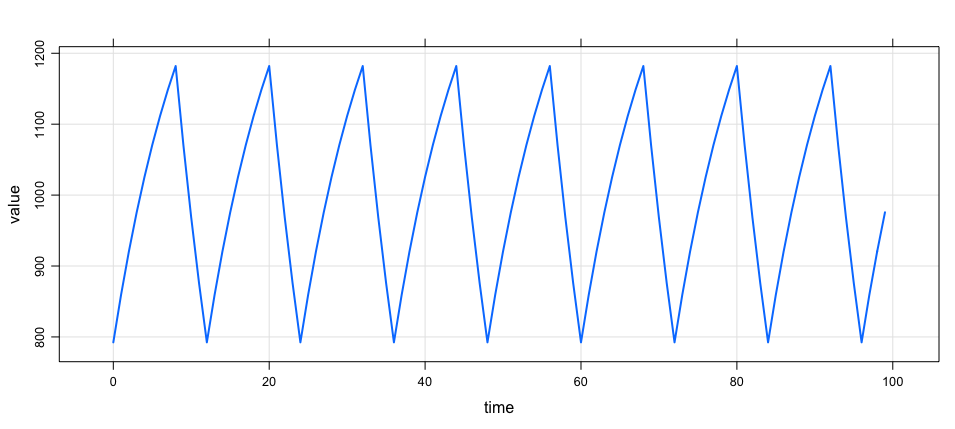
\includegraphics[width = 5in, height = 2.5in, trim=0in 0in 0 0in]{graphics/SS.png}
\caption{Simulated drug mass in a patient's gut at steady state. \textit{Every 12 hours, a patient
receives a drug administration. After being under this drug regiment for a certain period of time, 
the patient's system reaches a steady state. In this particular simulation, the drug administration
corresponds to the infusion of 1200 mg over 8 hours. Figure generated with mrgsolve.}}
\label{fig:steadyState}
\end{center}
\end{figure}

The brute force method to calculate a steady state would be to simulate a dosing regimen
for an extended period of time. While this works well in certain settings, it is not very efficient,
and sometimes not precise. A better approach is to exploit the definition of the steady state.
Let us suppose a treatment repeats itself every $\tau$ hours. In figure~\ref{fig:steadyState},
$\tau$ corresponds to the inter-dose interval. Then, once steady state has been reached,
we have:
%
\begin{eqnarray}
y(t_0) = y(t_0 + \tau)
\end{eqnarray}
%
where $t_0$ corresponds to the beginning of a dosing interval. This expression corresponds 
to an algebraic equation. Our goal is to solve for $y(t_0)$, the drug amount once the
patient has reached steady state (at the end of a dosing interval).

For the one and two compartment model, the solution can be worked out analytically. Similarly,
in the linear case, we can write a solution using the matrix exponential. In the nonlinear
case, we require a numerical algebraic solver.

\subsubsection{Algebraic solver}

\texttt{Stan} implements an algebraic solver, which uses Powell's hybrid method \cite{Powell:1970},
based on an unsupported routine in \texttt{Eigen}.
We find the method to work well in pharmacometrics.
It is robust, but slow for certain problems.
How well it scales in high dimensions is unclear.
There is therefore interest in expanding the number tools available to solve algebraic equations,
notably by incorporating less robust but faster methods such as Newton's solver.

Solving any algebraic equation can be turned into a root-finding problem. That is we want
to solve $f(x^*, \theta) = 0$ for $x^* \in \mathbb{R}^N$ in the neighborhood of some starting 
point $x \in \mathbb{R}^N$, which often corresponds to an initial guess for the solution. Note we
made $f$ explicitly dependent on the model parameters which appear in the algebraic
equation, $\theta \in \mathbb{R}^K$.

As always, we need to compute the Jacobian matrix of the outputs with respect to the input
parameters $\theta$. Because the algebraic solver is an iterative algorithm,
using standard AD is neither robust, nor efficient.
As with ODEs, we can exploit the structure of the problem, in particular using the implicit function theorem.
A standard computer experiment demonstrates the latter method is orders of magnitude
faster than using standard AD. % \cite{MargossianAD:2018}.

Formally, given the function $f: X \times \Theta \mapsto Y$, the implicit function theorem
states that if $f$ satisfies certain regulatory conditions in a neighborhood of the
starting point $(x, \theta)$ the roots are given by implicit functions, $x^* = h(y)$, where
$h:\Theta \mapsto X$ satisfies $f(h(y), y) = 0$. This allows us to define the desired
Jacobian as $\partial h(y) / \partial y$. For more details and some generalizations,
see \cite{Bell:2008}.

The implicit function theorem does not give us $h$, but it explicitly constructs 
the Jacobian of $h(y)$, which is all we need!
Defining the two initial Jacobian matrices.
%
\begin{eqnarray*}
J_x(x, \theta) = \frac{\partial f}{\partial x} (x, \theta)
\end{eqnarray*}
%
and
%
\begin{eqnarray*}
J_\theta = \frac{\partial f}{\partial \theta} (x, \theta),
\end{eqnarray*}

then the Jacobian of the roots is given by
%
\begin{eqnarray*}
\frac{\partial h}{\partial \theta}(\theta) = - [J_x(h(\theta), \theta)]^{-1} J_y(h(\theta), \theta)
\end{eqnarray*}
%
provided $J_x$ is invertible.

The Jacobians $J_x$ and $J_\theta$ can be computed with AD,
given the expression for $f$ is known, and \texttt{Stan} provides a method for matrix division. 

The invertibility condition for $J_x$ places restrictions on the structure of the
original problem. In particular, recall $X = \mathbb{R}^N$ and $\Theta = \mathbb{R}^K$,
and let $Y = \mathbb{R}^M$. Then $J_x$ is a $M \times N$ matrix and is invertible
if and only if $M = N$. In other words, we need as many unknowns as equations in our
algebraic system. Even then, $J_x$ can become singular if the roots are not uniquely
defined and other pathologies occur. For additional details, see chapter 17 of the \textit{Stan Book}.

\section{Open-source code for \texttt{Torsten}}

The primary repository for \texttt{Torsten}, which includes documentations, examples,
and installation files, is \url{https://github.com/metrumresearchgroup/Torsten}.

Stan's \texttt{math} library is written in \texttt{C++}, which offers a great deal of speed and 
flexibility. The \texttt{Stan} language provides a very handy interface that allows us to focus 
on statistical modeling and saves us the trouble of doing extensive coding in \texttt{C++}.
%
At run time, a make file translates our \texttt{Stan} model into \texttt{C++}, which then gets compiled 
and executed. Accordingly, there are two steps to add a function to Stan: (1) write the 
procedure in \texttt{C++}, (2) expose the procedure to the language so users may use it in a 
Stan file.
%
\texttt{Stan} interfaces with higher level languages, such as \texttt{R} and \texttt{Python}. 
\texttt{Torsten} exists as a forked 
version of \texttt{math} and \texttt{stan}. Other repos remain unchanged.

Regularly, we merge \texttt{Stan}'s latest release into \texttt{Torsten}. \\


\textit{Modifications in math.} All \texttt{Torsten} files are located in 
the Torsten directory, under \texttt{stan/math}. The
code can be found on GitHub: \\ \url{https://github.com/metrumresearchgroup/math}. \\

\textit{Modifications in Stan.} We do further modifications in \texttt{Stan} to expose \texttt{Torsten}'s 
functions. We edit \texttt{function\_signatures.h} to expose \texttt{PKModelOneCpt}, \texttt{PKModelTwoCpt}, 
and \texttt{linOdeModel}. The general and mix ODE model functions are higher-order functions (i.e. they 
take another function as one of their arguments). They are exposed by directly modifying 
the grammar files, following closely the example of \texttt{integrate\_ode\_rk45} and \texttt{integrate\_ode\_bdf}.
The code can be found on GitHub: \url{https://github.com/metrumresearchgroup/stan}.


% \bibliographystyle{custom}
% \bibliographystyle{custom}
\bibliographystyle{apacite}
\bibliography{custom.bib}

\end{document}
